\chapter[Método]{Método}

O método utilizado será uma interpretação do processo proposto por \citeonline{fayyad1996data} para descoberta de conhecimento, onde a partir de currículos da Plataforma Lattes serão obtidos indicadores em redes de coautoria inter- e intra-áreas.

\begin{figure}[htpb]
   \centering
   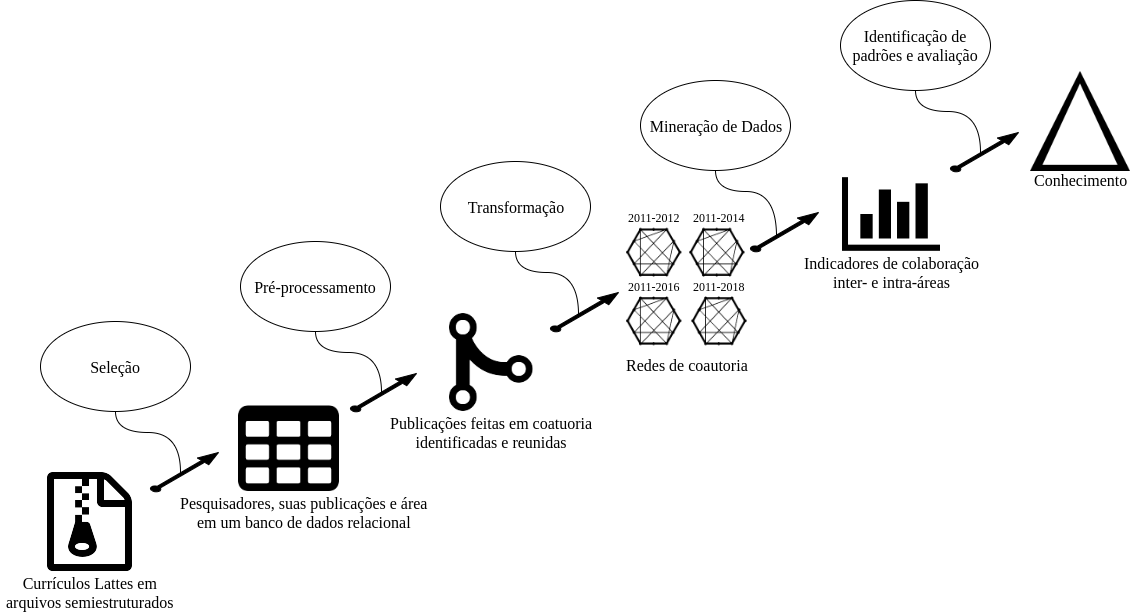
\includegraphics[scale=.3]{figs/fayyad-diagram-graph}
   \caption{Uma visão geral do processo de obtenção de indicadores para descoberta de conhecimento. Figura baseada no modelo proposto por \citeonline{fayyad1996data}.}
   \label{fig:processo}
\end{figure}

\section{Seleção}

Os currículos Lattes considerados neste projeto foram cedidos pelo Grupo de Pesquisa em Cientometria do CMCC/UFABC em arquivos no formato XML. Cada arquivo corresponde a um currículo com os dados do pesquisador.

Desses arquivos serão extraídas informações do pesquisador, \textit{e.g.}, nome completo, nome em citações bibliográficas, áreas de atuação, publicações científicas e data de última atualização do currículo. Todas as informações serão armazenadas em um banco de dados relacional.

\section{Pré-processamento}

Diversas produções científicas nessa área \cite{franceschet2011collaboration} \cite{mena2013prospecccao} \cite{reuther2006managing} descrevem casos onde uma publicação têm diversos nomes (sinônimos) e casos onde diferentes publicações possuem o mesmo nome (homônimos), cujos requerem tratamento a fim de obter um resultado mais confiável na etapa seguinte.

Neste trabalho, publicações sinônimas acontecem porque não foram cadastradas no currículo Lattes com exatamente a mesma informação, por exemplo, o mesmo título, haja vista que podem ocorrer abreviações de palavras, omissões de pontuação, ou erros de digitação. Neste caso, será utilizada uma abordagem com técnicas de distância de edição entre duas sequências de caracteres para deduplicar as publicações.

Publicações homônimas são mais difíceis de ocorrer pois é possível utilizar informações adicionais, e.g., autores, ano de publicação, revista, ou volume, para desambiguação.

Caso publicações homônimas não sejam identificadas corretamente, na próxima etapa será possível observar que a lista de coautores de um autor se dividirá em dois ou mais grupos altamente interconectados, mas sem colaborações entre grupos diferentes \cite{franceschet2011collaboration}. Ao detectar casos como este, poderá ser realizado tratamento manual.

\section{Transformação}

Usando as publicações obtidas nos currículos Lattes é possível identificar dois pesquisadores como coautores se uma mesma publicação aparece em seus currículos, e com isso construir uma rede de coautoria onde os nós são pesquisadores e os vértices a coautoria entre eles. O mesmo procedimento pode ser feito por períodos (\textit{e.g.}, biênio ou triênio), onde se obtém uma série de redes de coautoria com espaçamento temporal.

Nesta etapa pretendemos utilizar estruturas de dados eficientes para representar as redes de coautoria.

\section{Mineração de dados}

Nesta etapa serão feitos os cálculos de indicadores das redes de coautoria, onde planeja-se considerar as seguintes métricas topológicas: distância média, centralidade de grau, centralidade de proximidade, centralidade de autovetor, centralidade de contribuição, PageRank e AuthorRank \footnote{O AuthorRank é definido como uma medida que descreve as interações de um autor na rede de coautoria \cite{liu2005co}.}.

Pretendemos ainda, explorar novos arcabouços computacionais para processar todos os dados coletados.

\section{Identificação de padrões e avaliação}

Será determinada a existência de alguma correlação entre os indicadores obtidos e a análise desses indicadores para determinar se existe influência (ou impacto relativo) da Ciência da Computação em outras áreas.

Complementarmente, acontecimentos históricos que possam justificar o padrão encontrado serão buscados a fim de contextualizar a avaliação.

Diferentes conceitos de aprendizado de máquina e reconhecimento estatístico de padrões serão abordados.
